\subsection{Design for context variability}

We adopt goal modeling proposed by xxx and used in Tropos methodology. Tropos use a modeling framework based on i* \cite{yu_modelling_1996} which proposes the concepts of actor, goal, plan, resource and social dependency to model both the system-to-be and its organizational operating environment \cite{bresciani_tropos:_2004} \cite{morandini_tropos_2014}.

Key concepts in the Tropos metamodel are:

\begin{description}%[leftmargin=6em,style=nextline]
  \item[Actor] an entity that has strategic goals and intentionality

  \item[Agent] physical manifestation of an actor.

  \item[Goals] it represents actors’ strategic interests. \emph{Hard goals} are goals that have clear-cut criteria for deciding whether they are satisfied or not. \emph{Softgoals} have no clear-cut criteria and are normally used to describe preferences and quality-of-service demands.

  \item[Plan] it represents, at an abstract level, a way of doing something. The execution of a plan can be a means for satisfying a goal or for \emph{satisficing} (i.e. sufficiently satisfying) a softgoal.

  \item[Resource]  it represents a physical or an informational entity.

  \item[Dependency] it is a relationship between two actors that specify that one actor (the \emph{depended}) have a dependency to another actor (the \emph{dependee}) to attain some goal, execute some plan or deliver a resource. The object of the dependence is the \emph{dependum}.

  \item[Capability] it represents both the \emph{ability} of an actor to perform some action and the \emph{opportunity} of doing this.

  %\item[Belief] it represents actor knowledge of the world.

\end{description}

In Tropos requirements are represented as actors goals that are successively refined by AND/OR refinements. There are usually different ways to achieve a goal, and this is captured in goal models through multiple OR refinements.

An OR-refinement of a goal introduces a \emph{variation point} \cite{yu_goals_2008}.
Firgure \ref{fig:goal_model_example} shows an example of a goal model for "exemple system". The system goals is decomposed by means of AND/OR refinements. The \emph{variation point} \cite{yu_goals_2008} are shown.

\begin{figure}
  \centering
  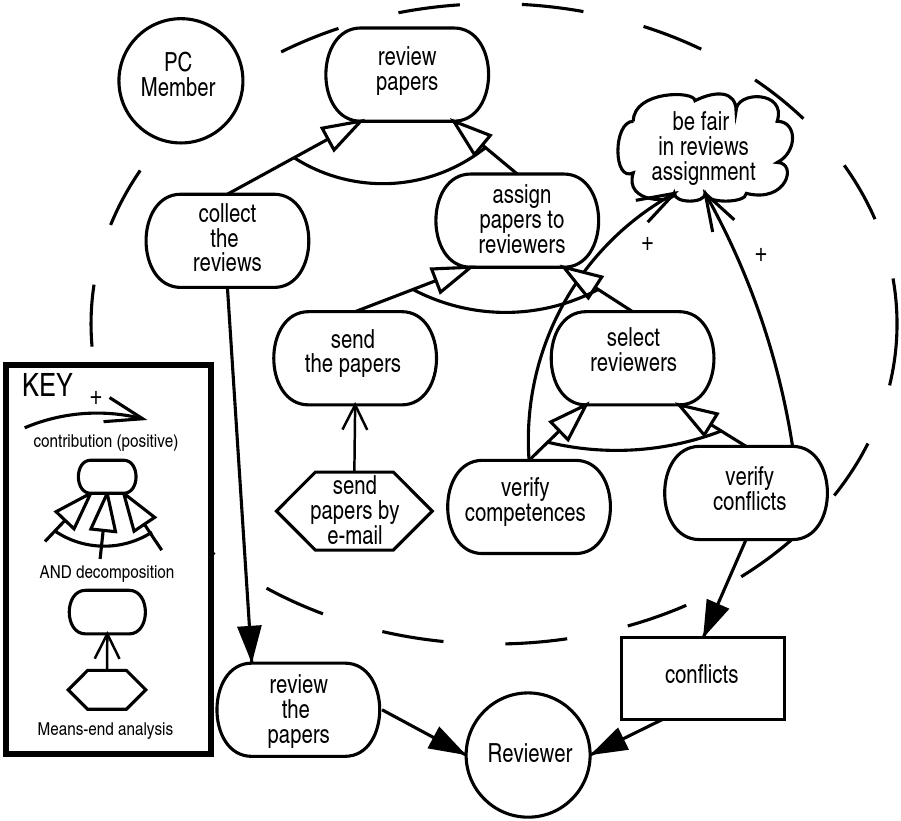
\includegraphics[width=1\linewidth]{refs/tropos_example_lr}
  \caption{\emph{Tropos} Goals Diagram}
  \label{fig:goal_model_example}
\end{figure}

\emph{Variability} is defined as all posible combinations of the choices in the variation points\cite{yu_goals_2008}.
